\documentclass[12pt, a4paper]{article}
\usepackage{epsfig}
\usepackage{subfigure}
%\usepackage{amscd}
\usepackage{amssymb}
\usepackage{amsbsy}
\usepackage{amsthm}
%\usepackage[dvips]{graphicx}
\usepackage{framed}
\usepackage{amsmath}

\usepackage{graphicx}

\usepackage{natbib}
\bibliographystyle{chicago}
%\usepackage{vmargin}
%\usepackage{index}
% left top textwidth textheight headheight
% headsep footheight footskip
%\setmargins{3.0cm}{2.5cm}{15.5 cm}{22cm}{0.5cm}{0cm}{1cm}{1cm}
\renewcommand{\baselinestretch}{1.5}
\pagenumbering{arabic}
\theoremstyle{plain}
\newtheorem{theorem}{Theorem}[section]
\newtheorem{corollary}[theorem]{Corollary}
\newtheorem{ill}[theorem]{Example}
\newtheorem{lemma}[theorem]{Lemma}
\newtheorem{proposition}[theorem]{Proposition}
\newtheorem{conjecture}[theorem]{Conjecture}
\newtheorem{axiom}{Axiom}
\theoremstyle{definition}
\newtheorem{definition}{Definition}[section]
\newtheorem{notation}{Notation}
\theoremstyle{remark}
\newtheorem{remark}{Remark}[section]
\newtheorem{example}{Example}[section]
\renewcommand{\thenotation}{}
\renewcommand{\thetable}{\thesection.\arabic{table}}
\renewcommand{\thefigure}{\thesection.\arabic{figure}}

%opening
\title{Residual Analysis for Linear and LME Models with \texttt{R}}
\author{Dublin \texttt{R}}





\begin{document}

\maketitle

\tableofcontents
\newpage
%--------------------------------------------------------------------------------------%
\section{Model Validation}
%http://www.itl.nist.gov/div898/handbook/pmd/section4/pmd44.htm
Model validation is possibly the most important step in the model building sequence. It is also one of the most overlooked. Often the validation of a model seems to consist of nothing more than quoting the $R^2$ statistic from the fit (which measures the fraction of the total variability in the response that is accounted for by the model). 

Unfortunately, a high $R^2$ value does not guarantee that the model fits the data well. Use of a model that does not fit the data well cannot provide good answers to the underlying engineering or scientific questions under investigation.



Model diagnostic techniques determine whether or not the distributional assumptions are satisfied, and to assess the influence of unusual observations.


\subsection{Why Use Residuals?}

If the model fit to the data were correct, the residuals would approximate the random errors that make the relationship between the explanatory variables and the response variable a statistical relationship. Therefore, if the residuals appear to behave randomly, it suggests that the model fits the data well. On the other hand, if non-random structure is evident in the residuals, it is a clear sign that the model fits the data poorly. 

The subsections listed below detail the types of plots to use to test different aspects of a model and give guidance on the correct interpretations of different results that could be observed for each type of plot.
%------------------------------------------------------------------------------------------------------------------------ %
\section{Introduction to Residuals}

The difference between the observed value of the dependent variable (y) and the predicted value ($\hat{y}$) is called the \textbf{residual} (e). Each data point has one residual.

\[\mbox{Residual} = \mbox{Observed value} - \mbox{Predicted value}\] 
\[e = y - \hat{y}\]

Both the sum and the mean of the residuals are equal to zero. 
%That is, Σ e = 0 and e = 0.

\subsection{Residual Plots}
A residual plot is a graph that shows the residuals on the vertical axis and the independent variable on the horizontal axis. If the points in a residual plot are randomly dispersed around the horizontal axis, a linear regression model is appropriate for the data; otherwise, a non-linear model is more appropriate.

Below the table on the left shows inputs and outputs from a simple linear regression analysis, and the chart on the right displays the residual (e) and independent variable (X) as a residual plot.

%x	60	70	80	85	95
%y	70	65	70	95	85
%ŷ	65.411	71.849	78.288	81.507	87.945
%e	4.589	-6.849	-8.288	13.493	-2.945
% Image of residual plot
\newpage
The residual plot shows a fairly random pattern - the first residual is positive, the next two are negative, the fourth is positive, and the last residual is negative. This random pattern indicates that a linear model provides a decent fit to the data.

Below, the residual plots show three typical patterns. The first plot shows a random pattern, indicating a good fit for a linear model. The other plot patterns are non-random (U-shaped and inverted U), suggesting a better fit for a non-linear model.

		
%Random pattern	Non-random: U-shaped	Non-random: Inverted U
In the next lesson, we will work on a problem, where the residual plot shows a non-random pattern. And we will show how to "transform" the data to use a linear model with nonlinear data.

%----------------------------------------------------------------------------------------------%
\newpage
%http://blog.minitab.com/blog/adventures-in-statistics/why-you-need-to-check-your-residual-plots-for-regression-analysis
In the graph above, you can predict non-zero values for the residuals based on the fitted value. For example, a fitted value of 8 has an expected residual that is negative. Conversely, a fitted value of 5 or 11 has an expected residual that is positive.

The non-random pattern in the residuals indicates that the deterministic portion (predictor variables) of the model is not capturing some explanatory information that is “leaking” into the residuals. The graph could represent several ways in which the model is not explaining all that is possible. 

Possibilities include:

\begin{itemize}
\item A missing variable
\item A missing higher-order term of a variable in the model to explain the curvature
\item A missing interction between terms already in the model
\end{itemize}


Identifying and fixing the problem so that the predictors now explain the information that they missed before should produce a good-looking set of residuals!

In addition to the above, here are two more specific ways that predictive information can sneak into the residuals:

The residuals should not be correlated with another variable. If you can predict the residuals with another variable, that variable should be included in the model. In Minitab’s regression, you can plot the residuals by other variables to look for this problem.


\subsubsection{Autocorrelation} 
Adjacent residuals should not be correlated with each other (\textbf{autocorrelation}). If you can use one residual to predict the next residual, there is some predictive information present that is not captured by the predictors. Typically, this situation involves time-ordered observations. 

For example, if a residual is more likely to be followed by another residual that has the same sign, adjacent residuals are positively correlated. You can include a variable that captures the relevant time-related information, or use a time series analysis. 

\subsubsection{Durbin-Watson Test for Autocorrelated Errors}
The \textbf{\textit{Durbin-Watson} }procedure is commonly used to to test for autocorrelationof residuals.

\begin{framed}
\begin{verbatim}
attach(mtcars)
 FitMod <- lm(mpg~wt+cyl)

# library(car)
durbinWatsonTest(FitMod)

\end{verbatim}
\end{framed}
\begin{verbatim}
> durbinWatsonTest(FitMod)
 lag Autocorrelation D-W Statistic p-value
   1       0.1302185      1.671096   0.252
 Alternative hypothesis: rho != 0
\end{verbatim}
\newpage

% http://polisci.msu.edu/jacoby/icpsr/regress3/lectures/week3/11.Outliers.pdf
%---------------------------------------------------------------------------------------------%
\newpage
\section{Standardization and Studentization}
\subsection{Standardization} %1.4.1

A random variable is said to be standardized if the difference from its mean is scaled by its standard deviation. The residuals above have mean zero but their variance is unknown, it depends on the true values of $\theta$. Standardization is thus not possible in practice.

\subsection{Studentization} %1.4.2
Instead, you can compute studentized residuals by dividing a residual by an estimate of its standard deviation. 

\subsection{Internal and External Studentization} %1.4.3
If that estimate is independent of the $i-$th observation, the process is termed \emph{external studentization}`external studentization'. This is usually accomplished by excluding the $i-$th observation when computing the estimate of its standard error. If the observation contributes to the
standard error computation, the residual is said to be \emph{internally studentization}internally studentized.

Externally \emph{studentized residual} studentized residual require iterative influence analysis or a profiled residuals variance.

\subsection{Computation}%1.4.4

%The computation of internally studentized residuals relies on the diagonal entries of $\boldsymbol{V} (\hat{\theta})$ - $\boldsymbol{Q} (\hat{\theta})$, where $\boldsymbol{Q} (\hat{\theta})$ is computed as

\[ \boldsymbol{Q} (\hat{\theta}) = \boldsymbol{X} ( \boldsymbol{X}^{\prime}\boldsymbol{Q} (\hat{\theta})^{-1}\boldsymbol{X})\boldsymbol{X}^{-1} \]

\subsection{Pearson Residual}%1.4.5

Another possible scaled residual is the \index{Pearson residual} `Pearson residual', whereby a residual is divided by the standard deviation of the dependent variable. The Pearson residual can be used when the variability of $\hat{\beta}$ is disregarded in the underlying assumptions.


%-------------------------------------------------------------------------------------------%
\newpage
\section{Leverage and Influence}
\subsection{Influence}
The influence of an observation can be thought of in terms of how much the predicted scores for other observations would differ if the observation in question were not included. 

Cook's D is a good measure of the influence of an observation and is proportional to the sum of the squared differences between predictions made with all observations in the analysis and predictions made leaving out the observation in question. If the predictions are the same with or without the observation in question, then the observation has no influence on the regression model. If the predictions differ greatly when the observation is not included in the analysis, then the observation is influential.

\subsection{Interpreting Cook's Distance}
A common rule of thumb is that an observation with a value of Cook's D over 1.0 has too much influence. As with all rules of thumb, this rule should be applied judiciously and not thoughtlessly.

\subsection{Leverage}
% http://onlinestatbook.com/2/regression/influential.html
% Leverage
The leverage of an observation is based on how much the observation's value on the predictor variable differs from the mean of the predictor variable. The greater an observation's leverage, the more potential it has to be an influential observation. 

For example, an observation with a value equal to the mean on the predictor variable has no influence on the slope of the regression line regardless of its value on the criterion variable. On the other hand, an observation that is extreme on the predictor variable has the potential to affect the slope greatly.

\subsubsection{Calculation of Leverage (h)}
The first step is to standardize the predictor variable so that it has a mean of 0 and a standard deviation of 1. Then, the leverage (h) is computed by squaring the observation's value on the standardized predictor variable, adding 1, and dividing by the number of observations.


\subsection{Summary of Influence Statistics}
\begin{itemize}
\item	\textbf{Studentized Residuals} – Residuals divided by their estimated standard errors (like t-statistics). Observations with values larger than 3 in absolute value are considered outliers.
\item	\textbf{Leverage Values (Hat Diag)} – Measure of how far an observation is from the others in terms of the levels of the independent variables (not the dependent variable). Observations with values larger than $2(k+1)/n$ are considered to be potentially highly influential, where k is the number of predictors and n is the sample size.
\item	\textbf{DFFITS} – Measure of how much an observation has effected its fitted value from the regression model. Values larger than $2\sqrt{(k+1)/n}$ in absolute value are considered highly influential. %Use standardized DFFITS in SPSS.
\item	\textbf{DFBETAS} – Measure of how much an observation has effected the estimate of a regression coefficient (there is one DFBETA for each regression coefficient, including the intercept). Values larger than 2/sqrt(n) in absolute value are considered highly influential.
\\
The measure that measures how much impact each observation has on a particular predictor is DFBETAs The DFBETA for a predictor and for a particular observation is the difference between the regression coefficient calculated for all of the data and the regression coefficient calculated with the observation deleted, scaled by the standard error calculated with the observation deleted. 

\item	\textbf{Cook’s D} – Measure of aggregate impact of each observation on the group of regression coefficients, as well as the group of fitted values. Values larger than 4/n are considered highly influential.
\end{itemize}


\subsection{Influential Observations : DFBeta and DFBetas}
% http://stats.stackexchange.com/questions/22161/how-to-read-cooks-distance-plots
Cook's distance refers to how far, on average, predicted y-values will move if the observation in question is dropped from the data set. dfbeta refers to how much a parameter estimate changes if the observation in question is dropped from the data set. Note that with k covariates, there will be k+1 dfbetas (the intercept,$\beta_0$, and 1 $\beta$ for each covariate). Cook's distance is presumably more important to you if you are doing predictive modeling, whereas dfbeta is more important in explanatory modeling.

\subsection{Cook's Distance}
% Interpretation
% http://stats.stackexchange.com/questions/22161/how-to-read-cooks-distance-plots %
Some texts tell you that points for which Cook's distance is higher than 1 are to be considered as influential. Other texts give you a threshold of $4/N$ or $4/(N−k−1)$, where N is the number of observations and k the number of explanatory variables. In your case the latter formula should yield a threshold around 0.1 .

John Fox (1), in his booklet on regression diagnostics is rather cautious when it comes to giving numerical thresholds. He advises the use of graphics and to examine in closer details the points with "values of D that are substantially larger than the rest". According to Fox, thresholds should just be used to enhance graphical displays.

In your case the observations 7 and 16 could be considered as influential. Well, I would at least have a closer look at them. The observation 29 is not substantially different from a couple of other observations.

(1) Fox, John. (1991). Regression Diagnostics: An Introduction. Sage Publications.
\subsection{Leverage}
 leverage is a term used in connection with regression analysis and, in particular, in analyses aimed at identifying those observations that are far away from corresponding average predictor values. Leverage points do not necessarily have a large effect on the outcome of fitting regression models.

Leverage points are those observations, if any, made at extreme or outlying values of the independent variables such that the lack of neighboring observations means that the fitted regression model will pass close to that particular observation.[1]

Modern computer packages for statistical analysis include, as part of their facilities for regression analysis, various quantitative measures for identifying influential observations: among these measures is partial leverage, a measure of how a variable contributes to the leverage of a datum.

%-------------------------------------------------------------------------------------------%
\newpage
\section{Regression Diagnostics with \texttt{R} }
% http://www.statmethods.net/stats/rdiagnostics.html

An excellent review of regression diagnostics is provided in John Fox's aptly named \textit{Overview of Regression Diagnostics}. Dr. Fox's car package provides advanced utilities for regression modeling.

\begin{verbatim}
(1) Fox, John. (1991). Regression Diagnostics: An Introduction. Sage Publications.
\end{verbatim}

\begin{framed}
\begin{verbatim}
# Assume that we are fitting a multiple linear regression
# on the MTCARS data
library(car)
fit <- lm(mpg~disp+hp+wt+drat, data=mtcars)

\end{verbatim}
\end{framed}


\subsection{Outliers}

Assessment of Outliers can be carried out using the \texttt{outlierTest} function.

\begin{framed}
\begin{verbatim}
outlierTest(fit) # Bonferonni p-value for most extreme obs
qqPlot(fit, main="QQ Plot") #qq plot for studentized resid 
leveragePlots(fit) # leverage plots
\end{verbatim}
\end{framed}
\subsection{Added Variable Plots}
\begin{framed}
\begin{verbatim}
# added variable plots 
av.Plots(fit)
\end{verbatim}
\end{framed}

\subsection{Non-constant Error Variance}
\begin{framed}
\begin{verbatim}

# Evaluate homoscedasticity
# non-constant error variance test
ncvTest(FitMod)
# plot studentized residuals vs. fitted values 
spreadLevelPlot(FitMod)
\end{verbatim}
\end{framed}

\begin{verbatim}
> ncvTest(FitMod)
Non-constant Variance Score Test 
Variance formula: ~ fitted.values 
Chisquare = 3.330027    Df = 1     p = 0.06802577 
\end{verbatim}

%mtcarsSpreadLevel Plot here

\begin{figure}[h!]
\centering
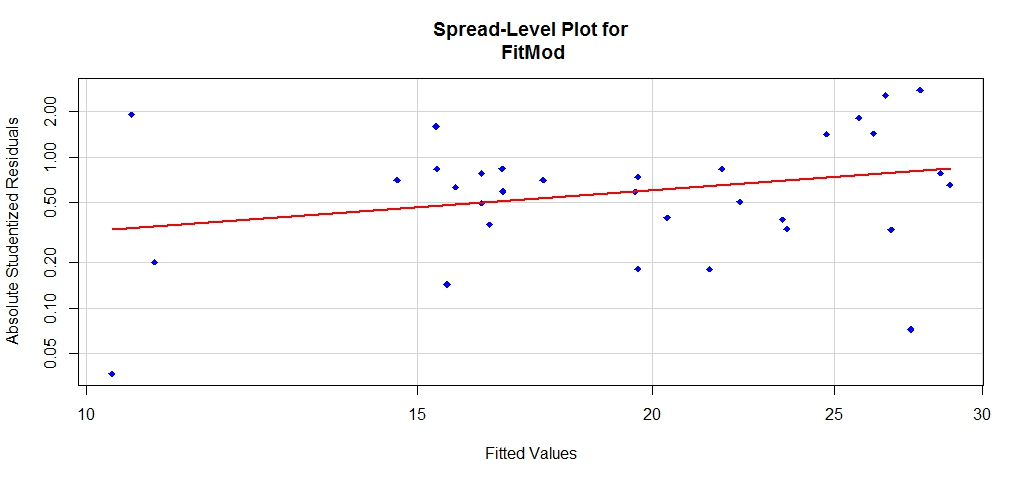
\includegraphics[width=0.7\linewidth]{./mtcarsSpreadLevelPlot}
\label{mtcarsSpreadLevelPlot}
\end{figure}


\begin{verbatim}
Suggested power transformation:  0.08866484 
\end{verbatim}

\subsection{Influential Observations}
\begin{framed}
\begin{verbatim}
# Influential Observations

# Cook's D plot
# identify D values > 4/(n-k-1) 
cutoff <- 4/((nrow(mtcars)-length(fit$coefficients)-2)) 
plot(fit, which=4, cook.levels=cutoff)
# Influence Plot 
influencePlot(fit,	 id.method="identify", main="Influence Plot", sub="Circle size is proportial to Cook's Distance" )
\end{verbatim}
\end{framed}
%-------------------------------------------------------------- %
\newpage
\section{Diagnostic Plots for Linear Models with \texttt{R}}
Plot Diagnostics for an \texttt{lm} Object

\subsection{Description}

Six plots (selectable by \texttt{which}) are currently available: 
\begin{enumerate}
\item a plot of residuals against fitted values, 
\item a Scale-Location plot of \textit{sqrt(| residuals |}) against fitted values, 
\item a Normal Q-Q plot, 
\item a plot of Cook's distances versus row labels, 
\item a plot of residuals against leverages, 
\item a plot of Cook's distances against leverage/(1-leverage).
\end{enumerate} By default, the first three and 5 are provided.
\newpage
%http://stats.stackexchange.com/questions/58141/interpreting-plot-lm
 I explained the assumption of homoscedasticity and the plots that can help you assess it (including scale-location plots [2]) on CV here: What does having constant variance in a linear regression model mean? I have discussed qq-plots [3] on CV here: QQ plot does not match histogram. So, what's left is primarily just understanding [5], the residual-leverage plot.

To understand this, we need to understand three things:

\begin{itemize}
\item leverage,
\item standardized residuals, and
\item Cook's distance.
\end{itemize}
%Move next bit to "Leverarge"
\subsubsection{Leverage}
To understand leverage, recognize that \textit{Ordinary Least Squares} regression fits a line that will pass through the centre of your data, ($\bar{x}, \bar{y}$). The line can be shallowly or steeply sloped, but it will pivot around that point like a lever on a fulcrum. We can take this analogy fairly literally: because OLS seeks to minimize the vertical distances between the data and the line, the data points that are further out towards the extremes of X will push / pull harder on the lever (i.e., the regression line); they have more leverage. One result of this could be that the results you get are driven by a few data points; that's what this plot is intended to help you determine.

% Standardization
Another result of the fact that points further out on X have more leverage is that they tend to be closer to the regression line (or more accurately: the regression line is fit so as to be closer to them) than points that are near $\bar{x}$. In other words, the residual standard deviation can differ at different points on X (even if the error standard deviation is constant). To correct for this, residuals are often standardized so that they have constant variance (assuming the underlying data generating process is homoscedastic, of course).

% Cook's Distance
One way to think about whether or not the results you have were driven by a given data point is to calculate how far the predicted values for your data would move if your model were fit without the data point in question. This calculated total distance is called \textbf{Cook's distance}. Fortunately, you don't have to rerun your regression model N times to find out how far the predicted values will move, Cook's D is a function of the leverage and standardized residual associated with each data point.

With these facts in mind, consider the plots associated with four different situations:
\begin{enumerate}
\item a dataset where everything is fine
\item a dataset with a high-leverage, but low-standardized residual point
\item a dataset with a low-leverage, but high-standardized residual point
\item a dataset with a high-leverage, high-standardized residual point
\end{enumerate}
\newpage
\subsection{Diagnostic Plots for LMs}
%-------------------------------------------------------------------------------------------%
\begin{itemize}
\item
The \textbf{Scale-Location} plot, also called ‘Spread-Location’ (or ‘S-L’ plot), takes the square root of the absolute residuals in order to diminish skewness (sqrt($|E|)$) is much less skewed than $| E |$ for Gaussian zero-mean E).

\item
The \textbf{Residual-Leverage} plot shows contours of equal Cook's distance, for values of \texttt{cook.levels} (by default 0.5 and 1) and omits cases with leverage one with a warning. If the leverages are constant (as is typically the case in a balanced aov situation) the plot uses factor level combinations instead of the leverages for the x-axis. \\
\textit{(The factor levels are ordered by mean fitted value.)}
\end{itemize}
\begin{framed}
\begin{verbatim}
plot(lm(mpg~wt+cyl),which=c(1),pch=18,col="red")
plot(lm(mpg~wt+cyl),which=c(2),pch=18,col="red")
plot(lm(mpg~wt+cyl),which=c(3),pch=18,col="red")
plot(lm(mpg~wt+cyl),which=c(4),pch=18,col="red")
plot(lm(mpg~wt+cyl),which=c(5),pch=18,col="red")
plot(lm(mpg~wt+cyl),which=c(6),pch=18,col="red")
\end{verbatim}
\end{framed}

\begin{figure}[h!]
\centering
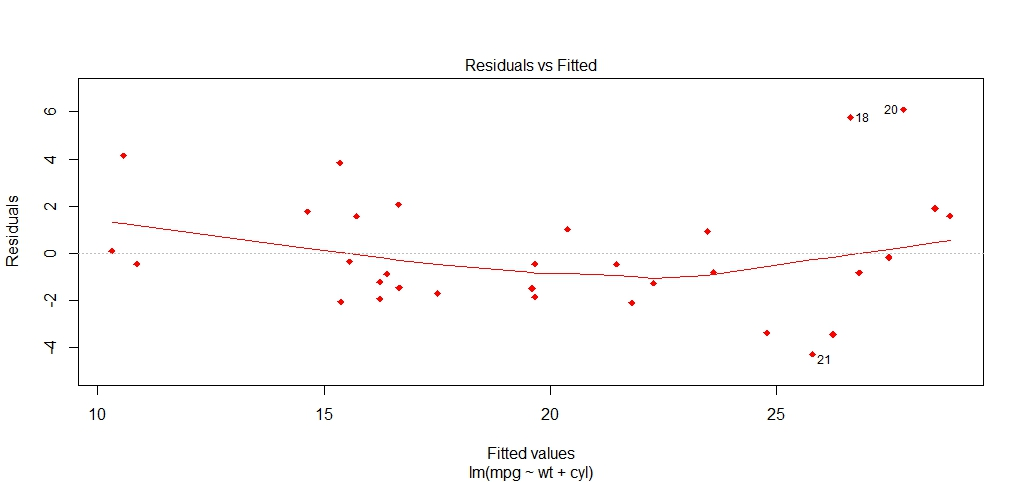
\includegraphics[width=0.9\linewidth]{./mtcarsDiagPlot1}

\label{mtcarsDiagPlot1}
\end{figure}

\newpage
\begin{figure}[h!]
\centering
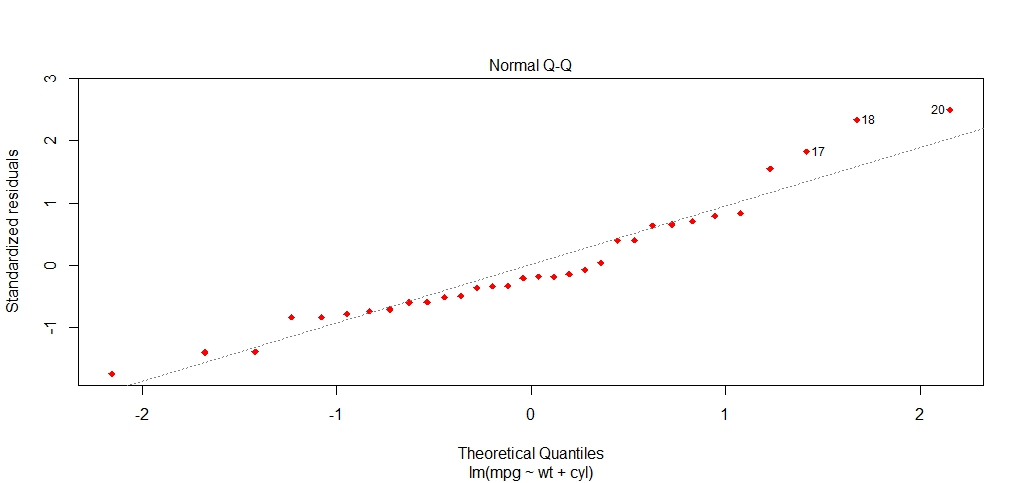
\includegraphics[width=0.9\linewidth]{./mtcarsDiagPlot2}

\label{mtcarsDiagPlot2}
\end{figure}

\subsubsection{Plot 3 : Normal Probability Plot}
This plot is used to assess the validity of the normality of the residuals.
\begin{figure}[h!]
\centering
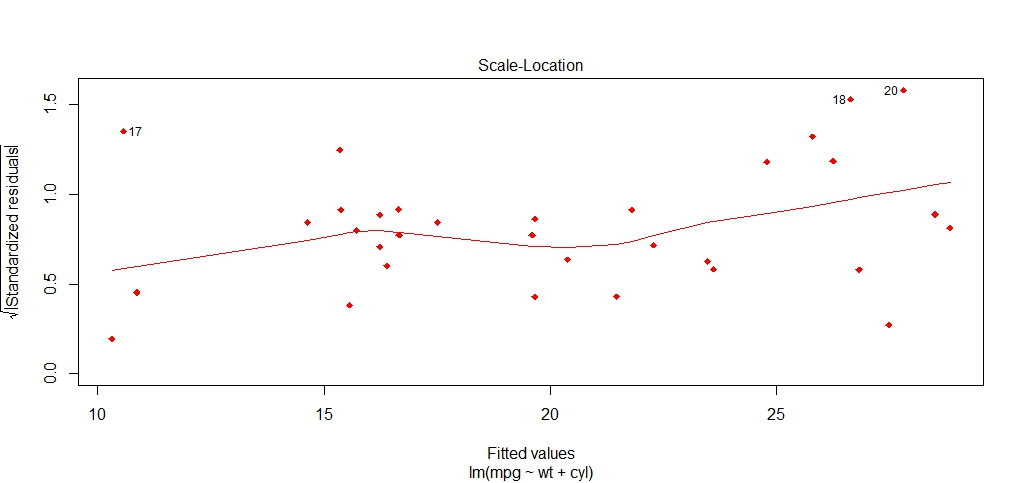
\includegraphics[width=0.9\linewidth]{./mtcarsDiagPlot3}

\label{mtcarsDiagPlot3}
\end{figure}

\newpage
\subsubsection{Plot 5 :  Cook's Distance}
\begin{figure}[h!]
\centering
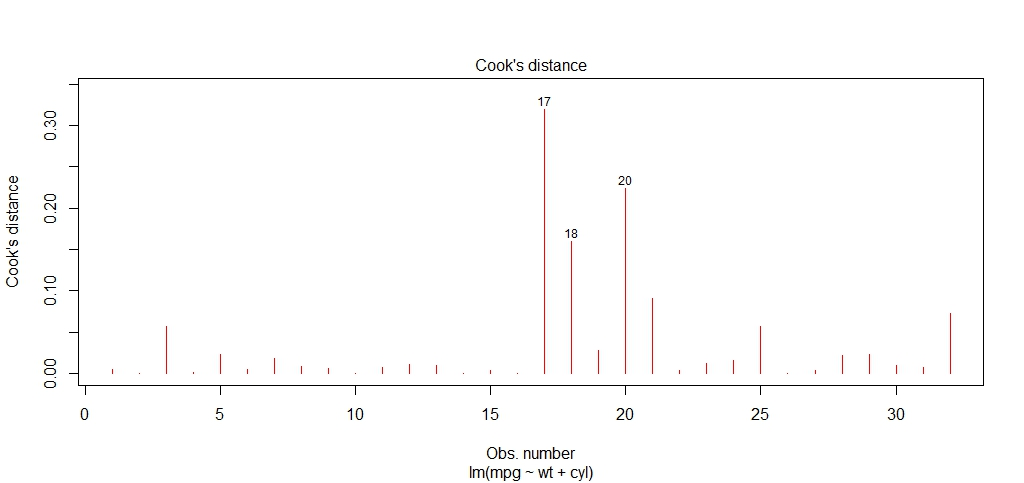
\includegraphics[width=0.9\linewidth]{./mtcarsDiagPlot4}

\label{mtcarsDiagPlot4}
\end{figure}


\begin{figure}[h!]
\centering
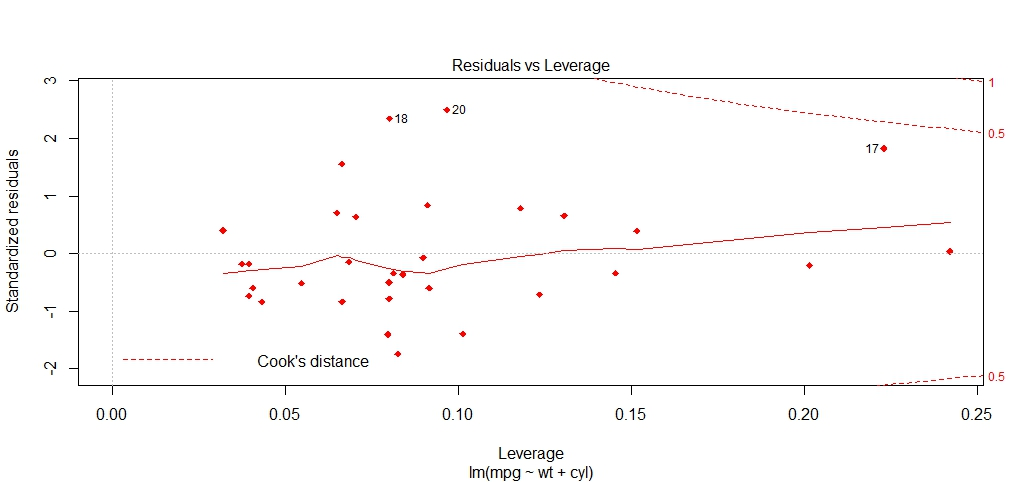
\includegraphics[width=0.9\linewidth]{./mtcarsDiagPlot5}

\label{mtcarsDiagPlot5}
\end{figure}


\subsubsection{Plot 6 :  Cook's Distance vs Leverage}
\begin{figure}[h!]
\centering
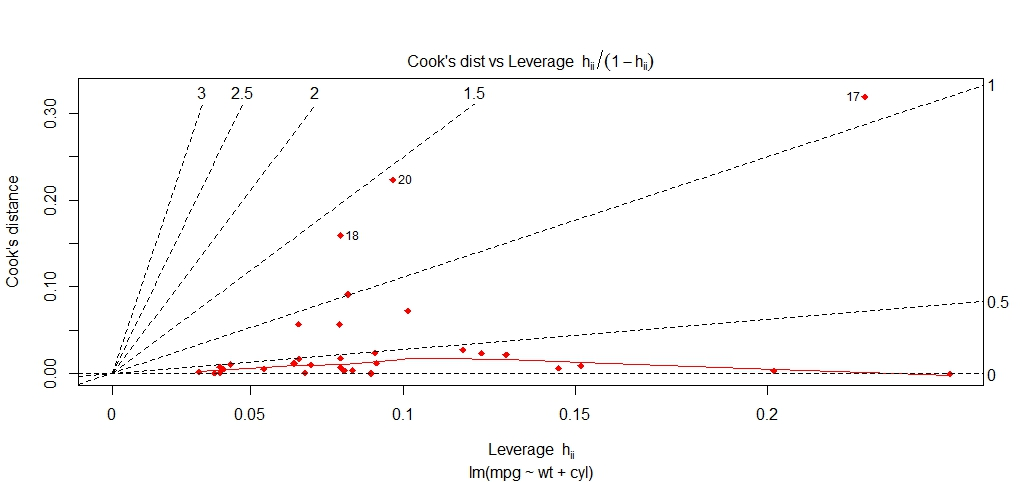
\includegraphics[width=0.9\linewidth]{./mtcarsDiagPlot6}

\label{mtcarsDiagPlot6}
\end{figure}


\begin{framed}
\begin{verbatim}
par(mfrow=c(4,1))
plot(fittedmodel)
par(opar)
\end{verbatim}
\end{framed}

% http://www.columbia.edu/~cjd11/charles_dimaggio/DIRE/resources/R/rFunctionsList.pdf

\newpage


\documentclass[main.tex]{subfiles}

% Load any packages needed for this document
\begin{document}
\section{Case Deletion} %1.14
Case-deleted analysis is a popular method for evaluating the influence of a subset of cases on inference.

\textbf{Cite: CPJ} develops case-deletion diagnostics for detecting influential observations in mixed linear models. Diagnostics for both fixed effects and variance components are proposed. Computational formulas are given that make the procedures feasible. The methods are illustrated using examples. 

\subsection{Case Deletion Diagnostic Statistics}
% http://support.sas.com/documentation/cdl/en/statug/63033/HTML/default/viewer.htm#statug_genmod_sect045.htm

For ordinary generalized linear models, regression diagnostic statistics developed by Williams (1987) are commonly used in statistical platforms such as SS. These diagnostics measure the influence of an individual observation on model fit, and generalize the one-step diagnostics developed by Pregibon (1981) for the logistic regression model for binary data.
Preisser and Qaqish (1996) further generalize regression diagnostics to apply to models for correlated data fit by generalized estimating equations (GEEs), where the influence of entire clusters of correlated observations is measured.


\subsection{Matrix Notation for  Case deletion notation} %1.14.1

For notational simplicity, $\boldsymbol{A}(i)$ denotes an $n \times m$ matrix $\boldsymbol{A}$ with the $i$-th row
removed, $a_i$ denotes the $i$-th row of $\boldsymbol{A}$, and $a_{ij}$ denotes the $(i, j)-$th element of $\boldsymbol{A}$.

\subsection{Partitioning Matrices} %1.14.2
Without loss of generality, matrices can be partitioned as if the $i-$th omitted observation is the first row; i.e. $i=1$.

%---------------------------------------------------------------------------%
\newpage
\subsection{CPJ's Three Propositions} %1.15
%-----------------------------%


\subsubsection{Proposition 1}

\[
\boldsymbol{V}^{-1} =
\left[ \begin{array}{cc}
\nu^{ii} & \lambda_{i}^{\prime}  \\
\lambda_{i} & \Lambda_{[i]}
\end{array}\right] \]


\[\boldsymbol{V}_{[i]}^{-1} = \boldsymbol{\Lambda}_{[i]} - { \lambda_{i} \lambda_{i} ^{\prime} \over \lambda_{i} } \]

%-----------------------------%
\subsection{Proposition 2}

\begin{itemize}
\item[(i)] $ \boldsymbol{X}_{[i]}^{T}\boldsymbol{V}^{-1}_{[i]}\boldsymbol{X}_{[i]}$ = $\boldsymbol{X}^{\prime}\boldsymbol{V}^{-1}\boldsymbol{X}$
\item[(ii)] = $(\boldsymbol{X}^{\prime}\boldsymbol{V}^{-1}\boldsymbol{Y})^{-1}$
\item[(iii)] $ \boldsymbol{X}_{[i]}^{T}\boldsymbol{V}^{-1}_{[i]}\boldsymbol{Y}_{[i]}$ = $\boldsymbol{X}^{\prime}\boldsymbol{V}^{-1}\boldsymbol{Y}$
\end{itemize}
%-----------------------------%
\subsection{Proposition 3}
This proposition is similar to the formula for the one-step Newtown Raphson estimate of the logistic regression coefficients given by Pregibon (1981) and discussed in Cook Weisberg.
\newpage
\section{Measures of Influence}
The impact of an observation on a regression fitting can be determined by the difference between the estimated regression coefficient of a model with all observations and the estimated coefficient when the particular observation is deleted. The measure DFBETA is the studentized value of this difference.

Influence arises at two stages of the LME model. Firstly when $V$ is estimated by $\hat{V}$, and subsequent
estimations of the fixed and random regression coefficients $\beta$ and $u$, given $\hat{V}$.

\subsection{Cook's Distance}
Cook's distance or Cook's D is a commonly used estimate of the influence of a data point when performing least squares regression analysis.

In a practical ordinary least squares analysis, Cook's distance can be used in several ways: to indicate data points that are particularly worth checking for validity; to indicate regions of the design space where it would be good to be able to obtain more data points. 

It is named after the American statistician R. Dennis Cook, who introduced the concept in 1977.

Cook's distance measures the effect of deleting a given observation. Data points with large residuals (outliers) and/or high leverage may distort the outcome and accuracy of a regression. Points with a large Cook's distance are considered to merit closer examination in the analysis.

\subsubsection{Computation}
\[ D_i = \frac{ \sum_{j=1}^n (\hat Y_j\ - \hat Y_{j(i)})^2 }{p \ \mathrm{MSE}} .\]
The following are the algebraically equivalent expressions (in case of simple linear regression):

\[ D_i = \frac{e_i^2}{p \ \mathrm{MSE}}\left[\frac{h_{ii}}{(1-h_{ii})^2}\right],\]
\[ D_i = \frac{ (\hat \beta - \hat {\beta}^{(-i)})^T(X^TX)(\hat \beta - \hat {\beta}^{(-i)}) } {(1+p)s^2}.\]
In the above equations:

\begin{itemize}
\item $\hat Y_j \,$ is the prediction from the full regression model for observation j;
\item $\hat Y_{j(i)}\,$ is the prediction for observation j from a refitted regression model in which observation i has been omitted;
\item $h_{ii} \,$ is the i-th diagonal element of the hat matrix 
\[ \mathbf{X}\left(\mathbf{X}^T\mathbf{X}\right)^{-1}\mathbf{X}^T;\]
\item $e_i \,$ is the crude residual (i.e., the difference between the observed value and the value fitted by the proposed model);
 \item $\mathrm{MSE} \,$ is the mean square error of the regression model;
\item $p$ is the number of fitted parameters in the model
\end{itemize}

\subsubsection{DFBETA}

The DFBETA statistic for measuring the influence of 
the th observation is defined as the one-step approximation to 
the difference in the MLE of the regression parameter vector and 
the MLE of the regression parameter vector without the th 
observation. This one-step approximation assumes a Fisher 
scoring step, and is given by

%EQUATION


\subsubsection{DFFITS} %1.16.1
DFFITS is a statistical measured designed to a show how influential an observation is in a statistical model. It is closely related to the studentized residual.
\begin{displaymath} DFFITS = {\widehat{y_i} -
\widehat{y_{i(k)}} \over s_{(k)} \sqrt{h_{ii}}} \end{displaymath}


\subsubsection{PRESS} %1.16.2
The prediction residual sum of squares (PRESS) is an value associated with this calculation. When fitting linear models, PRESS can be used as a criterion for model selection, with smaller values indicating better model fits.
\begin{equation}
PRESS = \sum(y-y^{(k)})^2
\end{equation}


\begin{itemize}
\item $e_{-Q} = y_{Q} - x_{Q}\hat{\beta}^{-Q}$
\item $PRESS_{(U)} = y_{i} - x\hat{\beta}_{(U)}$
\end{itemize}

\subsubsection{DFBETA} %1.16.3
\begin{eqnarray}
DFBETA_{a} &=& \hat{\beta} - \hat{\beta}_{(a)} \\
&=& B(Y-Y_{\bar{a}}
\end{eqnarray}
\end{document}
\input{RobustRegression.tex}



%-------------------------------------------------------------- %
\newpage
\section{Residual Analysis for GLMs (Optional Section)}





\subsection{Pearson and Deviance Residuals} 
% https://v8doc.sas.com/sashtml/insight/chap39/sect55.htm

Pearson Residuals





The Pearson residual is the raw residual divided by the square root of the variance function $V(\mu).$
The Pearson residual is the individual contribution to the Pearson $\chi^2$ statistic. 

For a binomial distribution with mi trials in the ith observation, it is defined as

\[ r_{Pi} = \sqrt{ m_{i}}
 \frac{r_{i}}{\sqrt{V(\hat{ \mu_{i}})}} \]
For other distributions, the Pearson residual is defined as

\[ r_{Pi} = \frac{r_{i}}{\sqrt{V(\hat{ \mu_{i}})}}\]
The Pearson residuals can be used to check the model fit at each observation for generalized linear models. 
%These residuals are stored in variables named RP_yname for each response variable, where yname is the response variable name. 
The standardized and studentized Pearson residuals are
\[
r_{Psi} = \frac{r_{Pi}}{\sqrt{\hat{ \phi} (1- h_{i})} } \]
\[ r_{Pti} = \frac{r_{Pi}}{\sqrt{ \hat{ \phi}_{(i)}
 (1- h_{i})} } \]



The \textbf{deviance residual} is the measure of deviance contributed from each observation and is given by
\[r_{Di} = \textrm{sign}( r_{i})
 \sqrt{ d_{i}}\]
where $d_i$ is the individual deviance contribution.
The deviance residuals can be used to check the model fit at each observation for generalized linear models. 

%These residuals are stored in variables named \textit{RD\_yname} for each response variable, where yname is the response variable name. 

The standardized and studentized deviance residuals are
\[
r_{Dsi} = \frac{r_{Di}}{\sqrt{\hat{ \phi} (1- h_{i})} }\]
\[r_{Dti} = \frac{r_{Di}}{\sqrt{ \hat{ \phi}_{(i)}
 (1- h_{i})}}\]
 
\newpage
 
\subsection{Diagnostics for Logistic Regression}

\subsection{Diagnostics for Poisson Regression}
%-------------------------------------------------------------- %
\newpage
\section{Residual Analysis for LME Models}
\subsection{Introduction}%1.1
In classical linear models model diagnostics have been become a required part of any statistical analysis, and the methods are commonly available in statistical packages and standard textbooks on applied regression. However it has been noted by several papers that model diagnostics do not often accompany LME model analyses.

\textbf{Cite:Zewotir} lists several established methods of analyzing influence in LME models. These methods include \begin{itemize}
\item Cook's distance for LME models,
\item \index{likelihood distance} likelihood distance,
\item the variance (information) ration,
\item the \index{Cook-Weisberg statistic} Cook-Weisberg statistic,
\item the \index{Andrews-Prebigon statistic} Andrews-Prebigon statistic.
\end{itemize}

%-------------------------------------------------------------------------------------------------------------------------------------%
\subsection{Zewotir Measures of Influence in LME Models}%2.2
%Zewotir page 161
\citet{Zewotir} describes a number of approaches to model diagnostics, investigating each of the following;
\begin{itemize}
\item Variance components
\item Fixed effects parameters
\item Prediction of the response variable and of random effects
\item likelihood function
\end{itemize}

\subsection{Cook's Distance applied to LMEs}
\begin{itemize}
\item For variance components $\gamma$: $CD(\gamma)_i$,
\item For fixed effect parameters $\beta$: $CD(\beta)_i$,
\item For random effect parameters $\boldsymbol{u}$: $CD(u)_i$,
\item For linear functions of $\hat{beta}$: $CD(\psi)_i$
\end{itemize}

\subsection{Iterative and non-iterative influence analysis for LMEs} %1.13

\textbf{Cite: Schabenberger} highlights some of the issue regarding implementing mixed model diagnostics.

A measure of total influence requires updates of all model parameters. However, this doesnt increase the procedures execution time by the same degree.

\subsection{Iterative Influence Analysis}

%----schabenberger page 8
For linear models, the implementation of influence analysis is straightforward.
However, for LME models, the process is more complex. Update formulas for the fixed effects are available only when the covariance parameters are assumed to be known. A measure of total influence requires updates of all model parameters. This can only be achieved in general is by omitting observations, then refitting the model.\textbf{Cite: Schabenberger} describes the choice between \index{iterative influence analysis} iterative influence analysis and \index{non-iterative influence analysis} non-iterative influence analysis.



%------------------------------------------------------------%
\begin{description}
\item[Random Effects]

A large value for $CD(u)_i$ indicates that the $i-$th observation is influential in predicting random effects.

\item[linear functions]
$CD(\psi)_i$ does not have to be calculated unless $CD(\beta)_i$ is large.


\item[Information Ratio]
\end{description}

%--------------------------------------------------------------%
\newpage
\section{Measures 2} %2.4

\subsection{Cook's Distance} %2.4.1
\begin{itemize}
\item For variance components $\gamma$
\end{itemize}

Diagnostic tool for variance components
\[ C_{\theta i} =(\hat(\theta)_{[i]} - \hat(\theta))^{T}\mbox{cov}( \hat(\theta))^{-1}(\hat(\theta)_{[i]} - \hat(\theta))\]

\subsection{Variance Ratio} %2.4.2
\begin{itemize}
\item For fixed effect parameters $\beta$.
\end{itemize}

\subsection{Cook-Weisberg statistic} %2.4.3
\begin{itemize}
\item For fixed effect parameters $\beta$.
\end{itemize}

\subsection{Andrews-Pregibon statistic} %2.4.4
\begin{itemize}
\item For fixed effect parameters $\beta$.
\end{itemize}
The Andrews-Pregibon statistic $AP_{i}$ is a measure of influence based on the volume of the confidence ellipsoid.
The larger this statistic is for observation $i$, the stronger the influence that observation will have on the model fit.


%---------------------------------------------------------------------------%




%------------------------------------------------------------%
\subsection{Likelihood Distance}


\citet{BA83}

\subsection{Diagnostics for LMEs with \texttt{R}}
influence.ME: Tools for detecting influential data in mixed effects models

influence.ME provides a collection of tools for detecting influential cases in generalized mixed effects models. It analyses models that were estimated using lme4. The basic rationale behind identifying influential data is that when iteratively single units are omitted from the data, models based on these data should not produce substantially different estimates. To standardize the assessment of how influential a (single group of) observation(s) is, several measures of influence are common practice, such as DFBETAS and Cook's Distance. In addition, we provide a measure of percentage change of the fixed point estimates and a simple procedure to detect changing levels of significance.


%------------------------------------------------------------------------------------------------%
% http://journal.r-project.org/archive/2012-2/RJournal_2012-2_Nieuwenhuis~et~al.pdf

You should have a look at the \texttt{R} package \textit{\textbf{influence.ME}}. It allows you to compute measures of influential data for mixed effects models generated by lme4.

An example model:
\begin{verbatim}
library(lme4)
model <- lmer(mpg ~ disp + (1 | cyl), mtcars)
\end{verbatim}

The function \texttt{influence} is the basis for all further steps:

\begin{verbatim}
library(influence.ME)
infl <- influence(model, obs = TRUE)
\end{verbatim}
Calculate Cook's distance:
\begin{verbatim}
cooks.distance(infl)
\end{verbatim}
Plot Cook's distance:
\begin{verbatim}
plot(infl, which = "cook")
\end{verbatim}
\newpage
%----------------------------------------------------------------------------------------%

\section{Case-Deletion Diagnostics for LMEs The CPJ Paper}%1.13

\subsection{Case-Deletion results for Variance components}
\textbf{Cite: CPJ}  examines case deletion results for estimates of the variance components, proposing the use of one-step estimates of variance components for examining case influence. The method describes focuses on REML estimation, but can easily be adapted to ML or other methods.

This paper develops their global influences for the deletion of single observations in two steps: a one-step estimate for the REML (or ML) estimate of the variance components, and an ordinary case-deletion diagnostic for a weighted regression problem ( conditional on the estimated covariance matrix) for fixed effects.

% Lesaffre's approach accords with that proposed by Christensen et al when applied in a repeated measurement context, with a large sample size.

\subsection{CPJ Notation} %1.13.1

\[ \boldsymbol{C} = \boldsymbol{H}^{-1} = \left[
\begin{array}{cc}
c_{ii} & \boldsymbol{c}_{i}^{\prime}\\
\boldsymbol{c}_{i} &  \boldsymbol{C}_{[i]}
\end{array} \right]
\]

\textbf{Cite: CPJ}  noted the following identity:

\[ \boldsymbol{H}_{[i]}^{-1}  = \boldsymbol{C}_{[i]} - {1 \over c_{ii}}\boldsymbol{c}_{[i]}\boldsymbol{c}_{[i]}^{\prime} \]


\textbf{Cite: CPJ} use the following as building blocks for case deletion statistics.
\begin{itemize}
\item $\breve{x}_i$
\item $\breve{z}_i$
\item $\breve{z}_ij$
\item $\breve{y}_i$
\item $p_ii$
\item $m_i$
\end{itemize}
All of these terms are a function of a row (or column) of $\boldsymbol{H}$ and $\boldsymbol{H}_{[i]}^{-1}$



\bibliographystyle{chicago}
\bibliography{DB-txfrbib}


\end{document} 
